\chapter{Structural Induction}
\section{Motivation}
Structural induction is used for reasoning about collections of objects, which are:
\begin{itemize}
    \item structured in a well defined way
    \item finite but can be arbitrarily large and complex
\end{itemize}

We can use this is reason about:
\begin{itemize}
	\item natural numbers
	\item data structures (lists, trees, etc)
	\item programs (can be large, but are finite)
	\item derivations of assertions like $E \Downarrow 4$ (finite trees of axioms and rules)
\end{itemize}

\section*{Structural Induction over Natural Numbers}
\[\mathbb{N} \in Nat ::= zero| succ(\mathbb{N})\]
To prove a property $P(\mathbb{N})$ holds, for every number $N \in Nat$ by induction on structure $\mathbb{N}$:
\begin{center}
    \begin{tabular}{l p{.8\textwidth}}
        \textbf{Base Case} & Prove $P(zero)$ \\
        \textbf{Inductive Case} & Prove $P(Succ(K))$ when $P(K)$ holds \\
    \end{tabular}
\end{center}
For example, we can prove the property:
\[plus(\mathbb{N}, zero) = \mathbb{N}\]
\subsubsection*{Base Case}
Show $plus(zero, zero) = zero$
\begin{center}
    \begin{tabular}{c r c l l}
        (1) & LHS & = & $plus(zero, zero)$ &                           \\
        (2) &     & = & $zero$             & (By definition of $plus$) \\
        (3) &     & = & RHS                & (As Required)             \\
    \end{tabular}
\end{center}

\subsubsection*{Inductive Case}
$N = succ(K)$
\\ Inductive Hypothesis $plus(K, zero) = K$
\\ Show $plus(succ(K), zero) = succ(K)$
\begin{center}
    \begin{tabular}{c r c l l}
        (1) & LHS & = & $plus(succ(K), zero)$                             \\
        (2) &     & = & $succ(plus(K, zero))$ & (By definition of $plus$) \\
        (3) &     & = & $succ(K)$             & (By Inductive Hypothesis) \\
        (4) &     & = & RHS                   & (As Required)             \\
    \end{tabular}
\end{center}
\noindent 
Mathematics induction is a special case of structural induction:
\[P(0) \land [\forall k \in \mathbb{N}. P(k) \Rightarrow P(k + 1)]\]
In the exam you may use $P(0)$ and $P(K+1)$ rather than $P(zero)$ and $P(succ(k))$ to save time.

\subsection{Binary Trees}
\[bTree \in BinaryTree ::= Node \ | \ Branch(bTree, bTree)\]
We can define a function $leaves$:
\[\begin{matrix*}[l]
    leaves(Node) & = 1 \\
    leaves(Branch(T_1, T_2)) & = leaves(T_1) + leaves(T_2) \\
\end{matrix*}\]
Or $branches$:
\[\begin{matrix*}[l]
    branches(Node) & = 0 \\
    branches(Branch(T_1,T_2)) & = branches(T_1) + branches(T_2) + 1 \\    
\end{matrix*}\]
    
\begin{examplebox}
    Prove By induction that $leaves(T) = branches(T) + 1$
    \tcblower
    \unfinished
\end{examplebox}

\section{Induction over SimpleExp}
To define a function on all expressions in \textit{SimpleExp}:
\begin{itemize}
	\item define $f(n)$ directly, for each number $n$.
	\item define $f(E_1 + E_2)$ in terms of $f(E_1)$ and $f(E_2)$.
	\item define $f(E_1 \times E_2)$ in terms of $f(E_1)$ and $f(E_2)$.
\end{itemize}

For example, we can do this with $den$:
\[den(E) = n \leftrightarrow E \Downarrow n\]

\subsection{Many Steps of Evaluation}
Given $\to$ we can define a new relation $\to^*$ as:
\[E \to^* E' \leftrightarrow (E = E' \lor E \to E_1 \to E_2 \to \dots \to E_k \to E')\]
For expressions, the final answer is $n$ if $E \to^* n$.
\subsection{Multi-Step Reductions}
The relation $E \to^n E'$ is defined using mathematics induction by:
\subsubsection{Base Case}
\[\forall E \in SImpleExp . \ [E \to^0 E]\]

\subsubsection{Inductive Case}
\[\forall E, E' \in SimpleExp . \ [E \to^{k+1} E' \Leftrightarrow \exists E'' . \ [E \to^k E'' \land E'' \to E']]\]

\subsubsection{Definition}
\[\forall E, E' . \ [E \to^* E' \Leftrightarrow \exists n.[E \to^n E']]\]
$\to^*$ - there are some number of steps to evaluate to $E'$

\subsection*{Properties of $\to$}
\begin{center}
    \begin{tabular}{l p{.8\textwidth}}
        \textbf{Determinacy}   & If $E \to E_1$ and $E \to E_2$ then $E_1 = E_2$. \\
        \textbf{Confluence}    & If $E \to^* E_1$ and $E \to^*E_2$ then there exists $E'$ such that $E_1 \to^* E'$ and $E_2 \to^* E'$. \\
        \textbf{Unique answer} & If $E \to^* n_1$ and $E \to^* n_2$ then $n_1 = n_2$. \\
        \textbf{Normal Forms}  & Normal form is numbers ($\mathbb{N}$) for any $E$, $E = n$ or $E \to E'$ for some $E'$. \\
        \textbf{Normalisation} & No infinite sequences of expressions $E_1,E_2,E_3, \dots$ such that for all $i \in \mathbb{N}$ $E_1 \to E_{i+1}$ (Every path goes to a normal form). \\
    \end{tabular}
\end{center}


\subsection{Confluence of Small Step}
We can prove a lemma expressing confluence:
\[L_1 : \forall n \in \mathbb{N} . \forall E, E_1, E_2 \in SimpleExp . [E \to^n E_1 \land E \to^* E_2 \Rightarrow \exists E' \in SimpleExp . [E_1 \to^* E' \land E_2 \to^* E']]\]
\subsubsection{Lemma $\Rightarrow$ Confluence}
Confluence is: $\forall E, E_1, E_2 \in SimpleExp . [E \to^* E_1 \land E \to^* E_2 \Rightarrow \exists E' \in SimpleExp . [E_1 \to^* E' \land E_2 \to^* E']]$
From lemma $L_1$
\begin{center}
	\begin{tabular}{l l l}
		(1) & Take some arbitrary $E, E_1, E_2 \in SimpleExp$, assume confluence holds. & (Initial Setup)                 \\
		(2) & $E \to^* E_1$                                                             & (By Confluence)                 \\
		(3) & $\exists n \in \mathbb{N} .[E \to^n E_1]$                                 & (By 2 \& definition of $\to^*$) \\
		(4) & Hence $L_1$                                                               & (By 3)                          \\
	\end{tabular}
\end{center}
\subsection{Determinacy of Small Step}
We create a property $P$:
\[P(E) \overset{def}{=} \forall E_1,E_2 \in SimpleExp .[E \to E_1 \land E \to E_2 \Rightarrow E_1 = E_2] \]
There are 3 rules that apply:
\[\begin{matrix}
		\whilestdef{A}{}{n_1 + n_2 \to n}{n = n_1 + n_2} & \whilestdef{B}{E \to E'}{n + E \to n + E'}{} & \whilestdef{C}{E_1 \to E_1'}{E_1 + E_2 \to E_1' + E_2}{}
	\end{matrix}\]
\subsubsection{Base Case}
Take arbitrary $n \in \mathbb{N}$ and $E_1,E_2 \in SimpleExp$ such that $n \to E_1 \land n \to E_2$ to show $E_1 = E_2$.
\begin{center}
	\begin{tabular}{l l l}
		(1) & $n \not\to$                                       & (By inversion on A,B \& C) \\
		(2) & $\neg (n \to E_1)$                                & (By 1)                     \\
		(3) & $\neg (n \to E_1 \land n \to E_2)$                & (By 2)                     \\
		(4) & $n \to E_1 \land n \to E_2 \Rightarrow E_1 = E_2$ & (By 3)                     \\
		(5) & $E \to E_1 \land E \to E_2 \Rightarrow E_1 = E_2$ & (By 4)                     \\
	\end{tabular}
\end{center}
Hence $P(n)$
\subsubsection{Inductive Step}
Take arbitrary $E, E_1,E_2$ such that $E = E_1 + E_2$
\\ Inductive Hypothesis:
\[IH_1 = P(E_1)\]
\[IH_2 = P(E_2)\]
Assume there exists $E_3, E_4 \in SimpleExp$ such that $E_1 + E_2 \to E_3$ and $E_1 + E_2 \to E_4$.
\\ To show $E_3 = E_4$.
\\
\\ From inversion on A, B \& C there are 3 cases to consider:
\\ \textbf{For A:}
\begin{center}
	\begin{tabular}{l l l}
		(1) & There exists $n_1, n_2 \in \mathbb{N}$ such that $E_1 = n_1$ and $E_2 = n_2$ & (By case A) \\
		(3) & $E_3 = n_1 + n_2$                                                            & (By 1, A)   \\
		(4) & $E_4 = n_1 + n_2$                                                            & (By 1, A)   \\
		(5) & $E_3 = E_4$                                                                  & (By 3 \& 4) \\
	\end{tabular}
\end{center}
\textbf{For B:}
\begin{center}
	\begin{tabular}{l l l}
		(1) & There exists $n \in \mathbb{N}$ such that $E_1 = n$      & (By case B)   \\
		(2) & There exists $E' \in SimpleExp$ such that $E_2 \to E'$   & (By case B)   \\
		(3) & $E_3 = n + E'$                                           & (By case B)   \\
		(4) & There exists $E'' \in SimpleExp$ such that $E_2 \to E''$ & (By case B)   \\
		(5) & $E_4 = n + E''$                                          & (By case B)   \\
		(6) & $E' = E''$                                               & (By $IH_2$)   \\
		(7) & $E_3 = E_4$                                              & (By 3,5 \& 6) \\
	\end{tabular}
\end{center}
\textbf{For C:}
\begin{center}
	\begin{tabular}{l l l}
		(1) & There exists $E' \in SimpleExp$ such that $E_1 \to E'$   & (By case C)   \\
		(2) & There exists $E'' \in SimpleExp$ such that $E_1 \to E''$ & (By case C)   \\
		(3) & $E_3 = E' + E_2$                                         & (By case C)   \\
		(4) & $E_4 = E'' + E_2$                                        & (By case C)   \\
		(5) & $E' = E''$                                               & (By $IH_1$)   \\
		(6) & $E_3 = E_4$                                              & (By 3,4 \& 5)
	\end{tabular}
\end{center}
(If $E$ reduces to $E_1$ in $n$ steps, and to $E_2$ in some number of steps, then there must be some $E'$ that $E_1$ and $E_2$ reduce to.)
\subsubsection*{Base Case}
The base cases has $n=0$. Hence $E = E_1$, and hence $E_1 \to^* E_2$ and $E_1 \to^* E'$
\begin{center}
	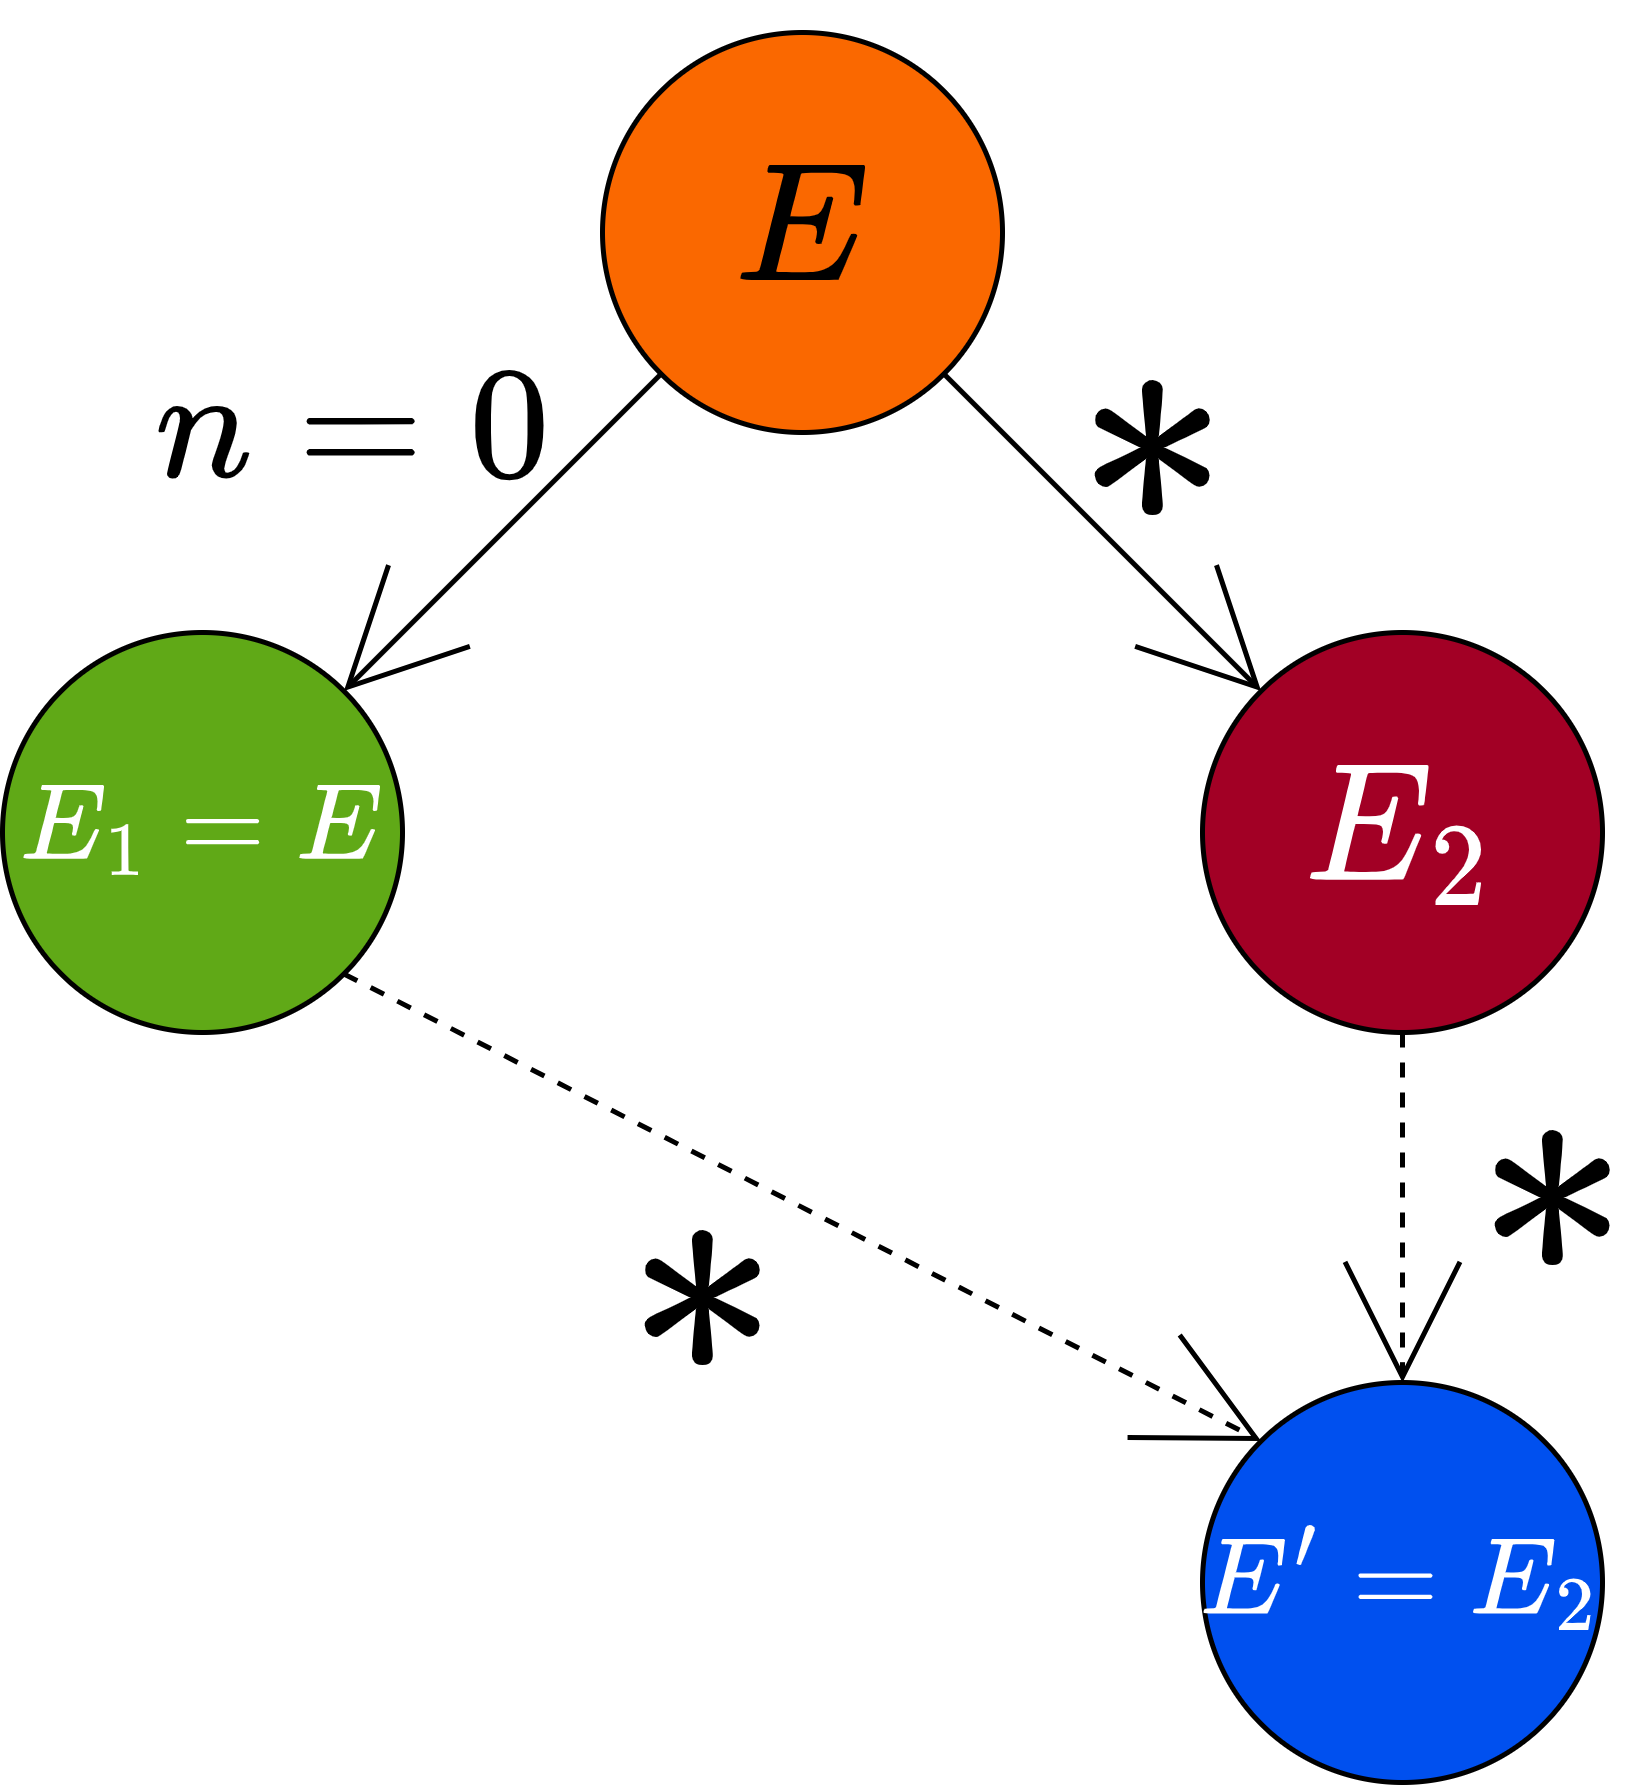
\includegraphics[scale=0.1]{structural_induction/images/confluence_base_case.drawio.png}
\end{center}
\subsubsection*{Inductive Case}
Next we assume confluence for up to $k$ steps, and attempt to prove for $k+1$ steps.
\begin{center}
	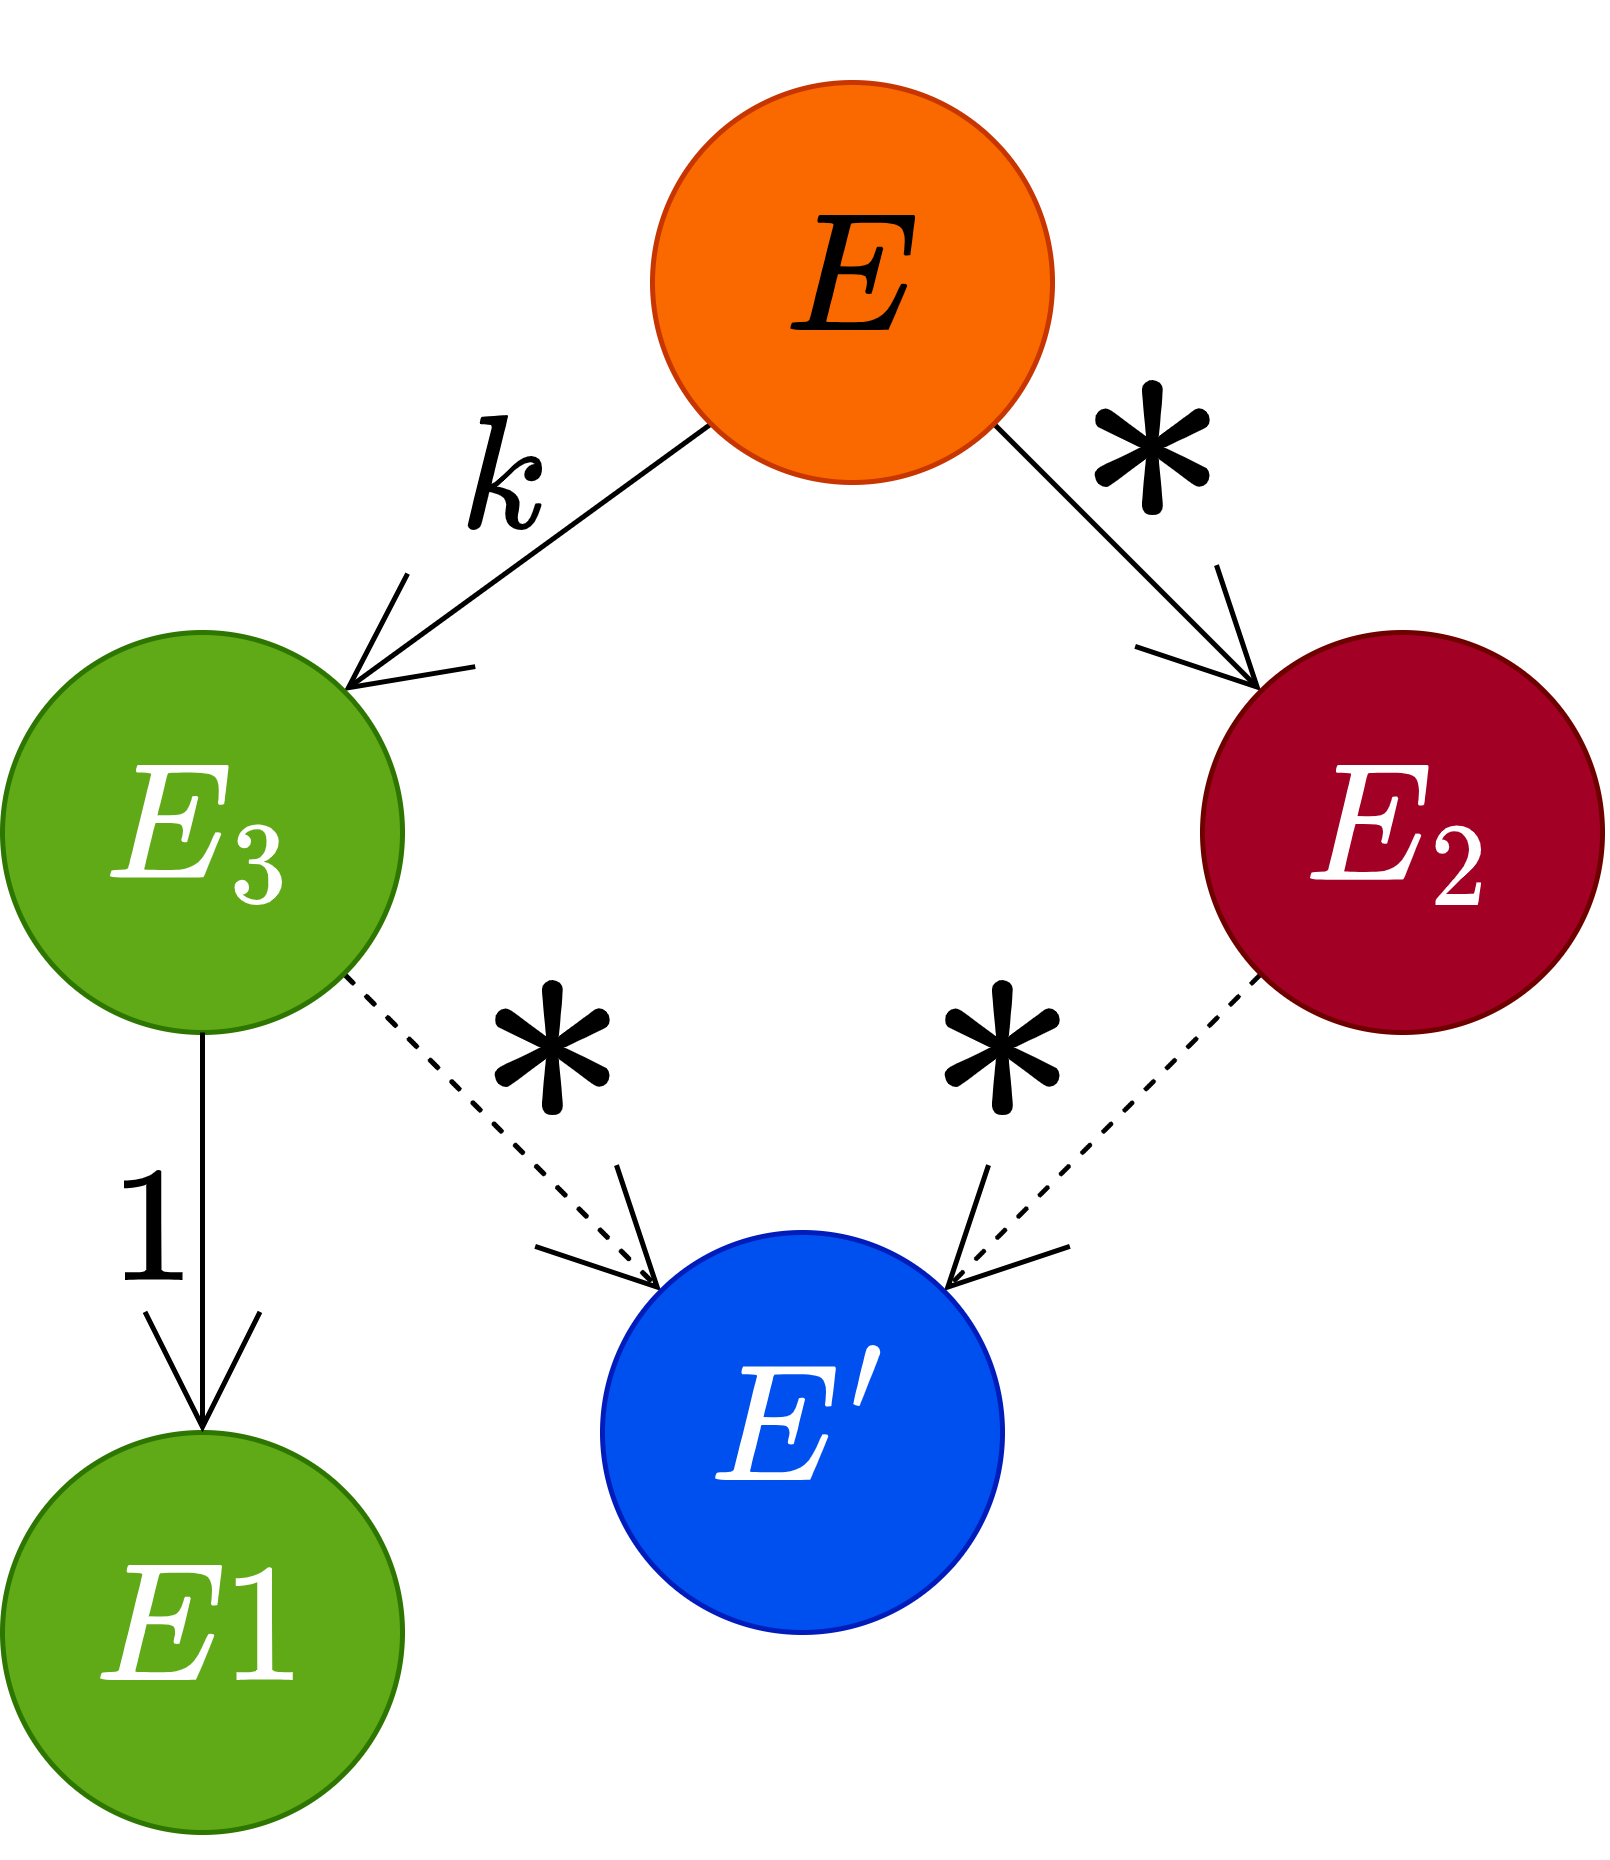
\includegraphics[scale=0.1]{structural_induction/images/confluence_inductive_case.drawio.png}
\end{center}
We have two cases:
\\ \textbf{Case 1:} $E_3 = E'$, this is easy as $E_2 \to^* E' \to^0 E3 \to^1 E1$.
\begin{center}
	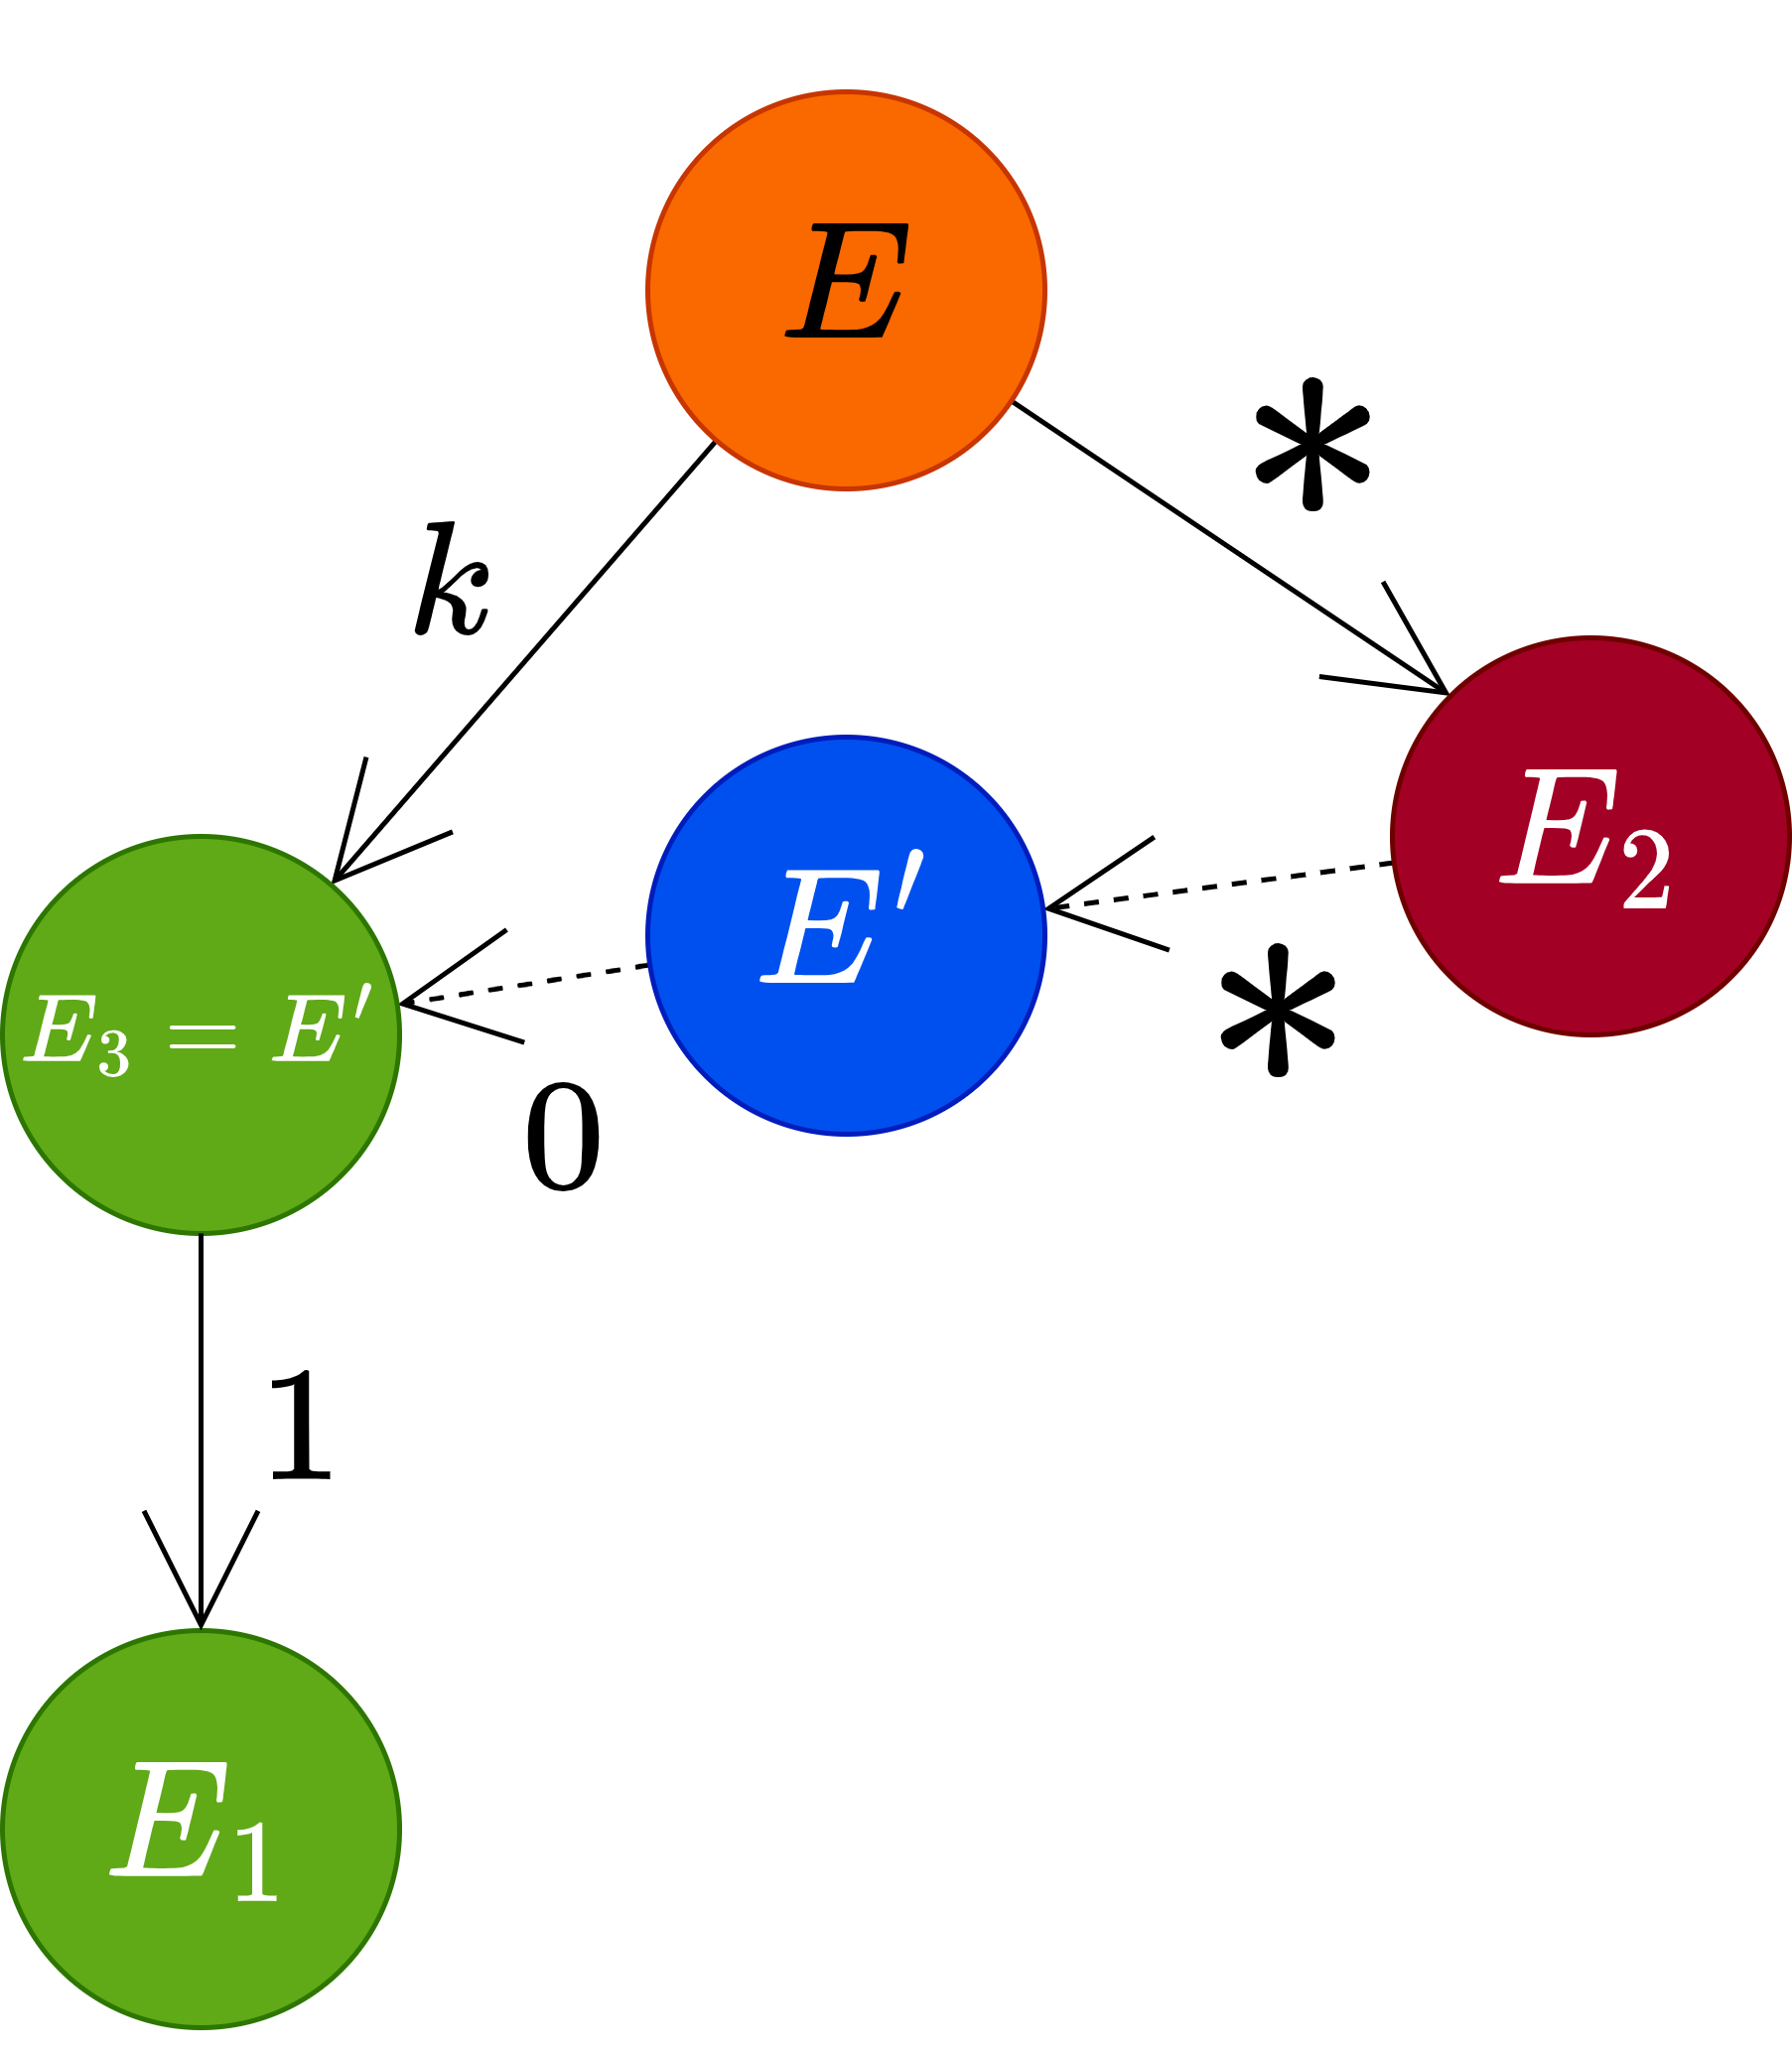
\includegraphics[scale=0.1]{structural_induction/images/confluence_inductive_case_A.drawio.png}
\end{center}
\textbf{Case 2:} $E_3 \to^1 E'' \to^* E'$, in this case as $E_3 \to^1 E1$ we know by determinacy that $E'' = E_1$ and hence $E_1 \to^* E'$.
\begin{center}
	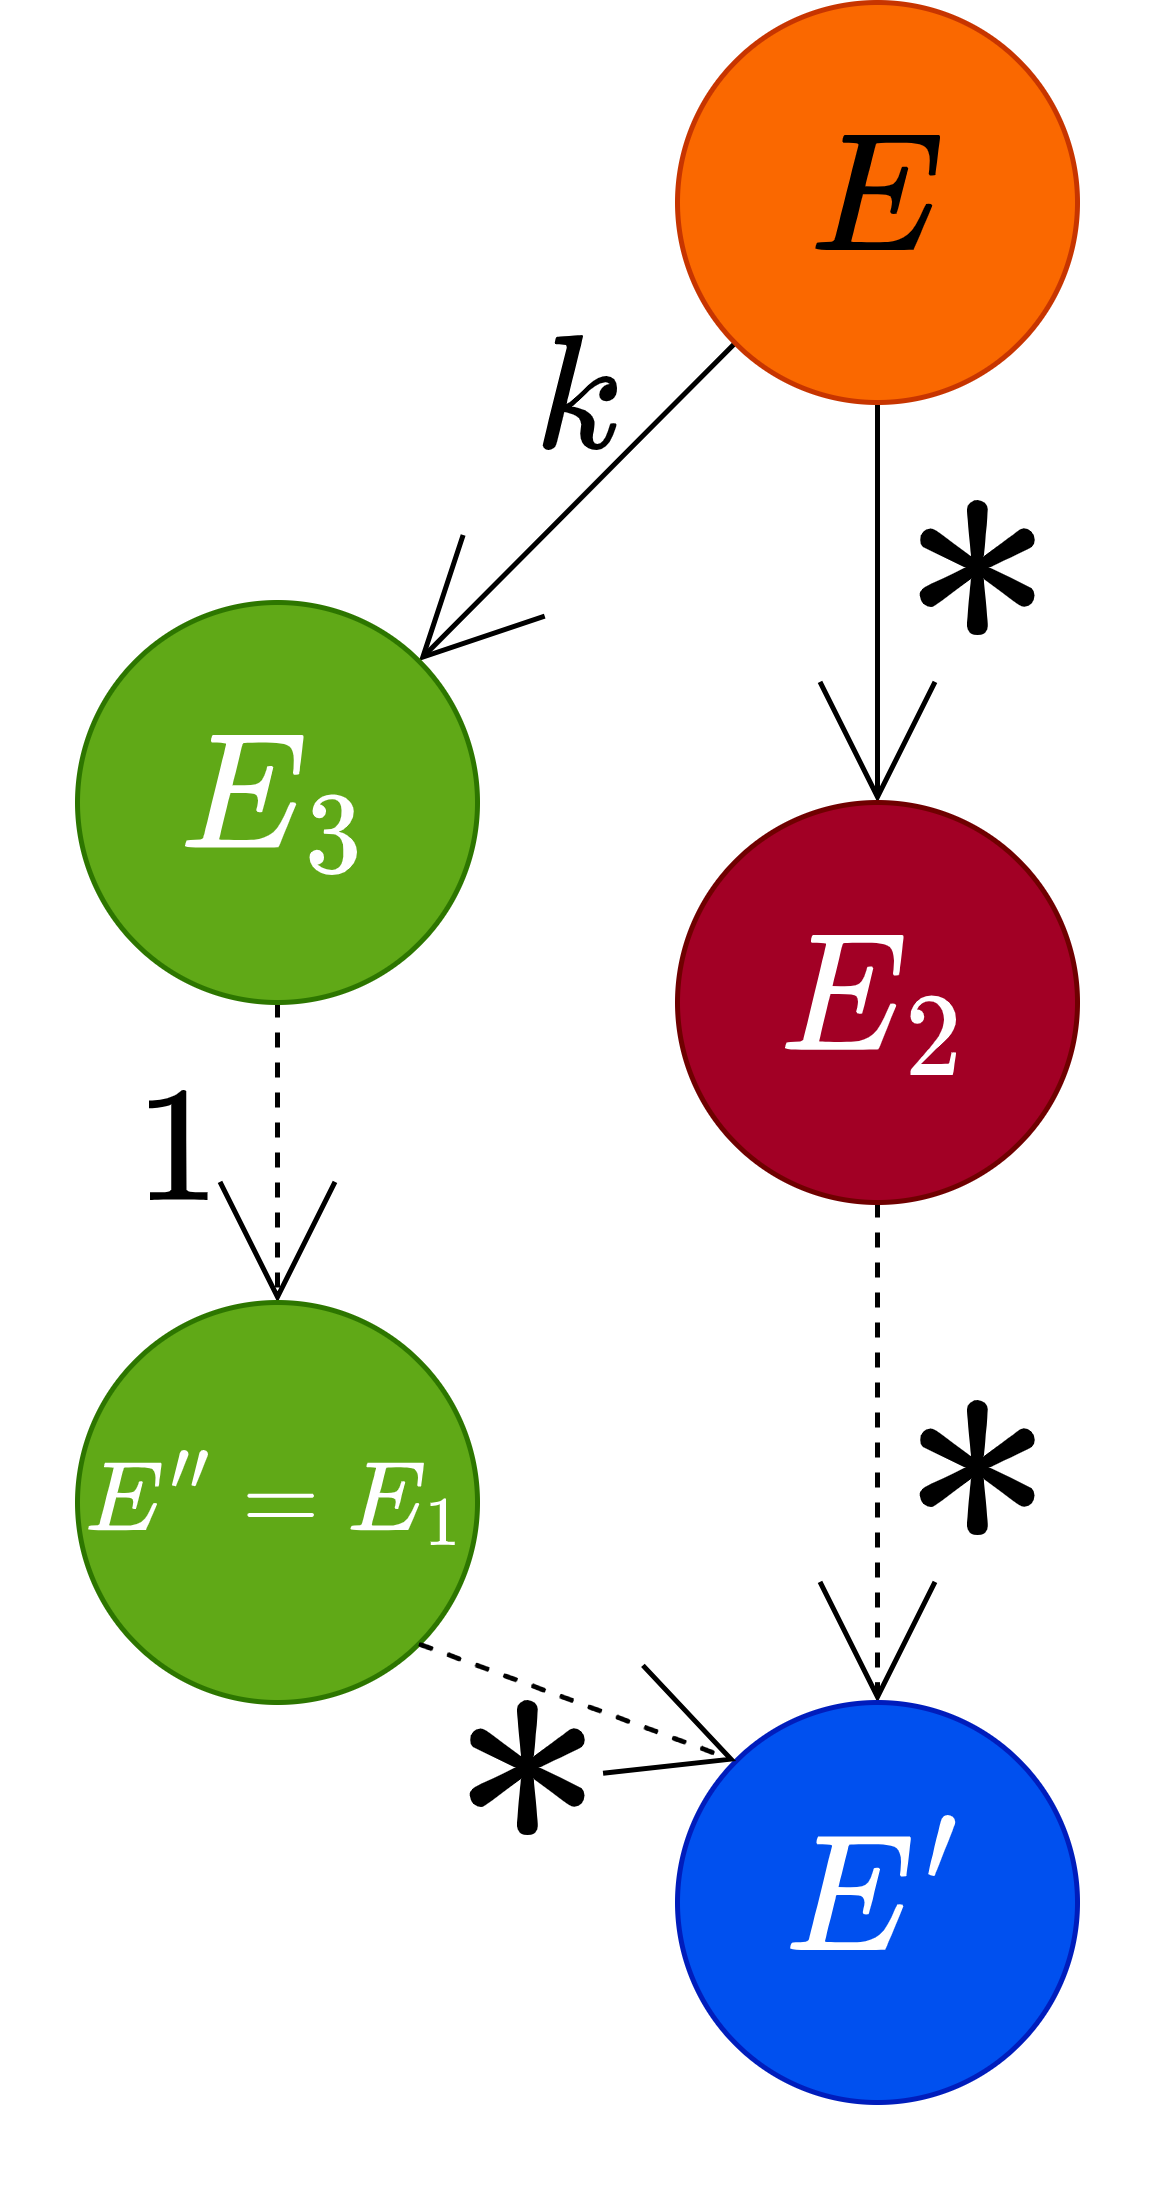
\includegraphics[scale=0.1]{structural_induction/images/confluence_inductive_case_B.drawio.png}
\end{center}


\section{Multi-Step Reductions}
\textit{Note: We will reference to state by set $State \triangleq (Var \rightharpoonup \mathbb{N})$.}

\begin{definitionbox}{Lemma}
	A small proven proposition that can be used in a proof. Used to make the proof smaller.
	\\
	\\ Also know as an "auxiliary theorem" or "helper theorem".
\end{definitionbox}
\begin{definitionbox}{Corollary}
	A theorem connected by a short proof to another existing theorem.
	\\
	\\ If B is can be easily deduced from A (or is evident in A's proof) then B is a corollary of A.
\end{definitionbox}
\subsection{Lemmas}
\begin{enumerate}
	\item $\forall r \in \mathbb{N}. \forall E_1,E_1',E_2 \in SimpleExp. [E_1 \to^r E_1' \Rightarrow (E_1 + E_2) \to^r (E_1' + E_2)]$
	\item $\forall r,n \in \mathbb{N}. \forall E_2,E_2' \in SimpleExp . [E_2 \to^r E_2' \Rightarrow (n + E_2) \to^r (n + E_2')]$
\end{enumerate}
\subsection{Corollaries}
\begin{enumerate}
	\item $\forall n_1 \in \mathbb{N} . \forall E_1, E_2 \in SimpleExp . [E_1 \to^* n_1 \Rightarrow (E_1 + E_2) \to^* (n_1 + E_2)]$
	\item $\forall n_1, n_2 \in \mathbb{N} . \forall E_2 \in SimpleExp . [E_2 \to^* n_2 \Rightarrow (n_1 + E_2) \to^* (n_1 + n_2)]$
	\item $\forall n,n_1, n_2, \in \mathbb{N} . \forall E_1, E_2 \in SimpleExp . [E_1 \to^* n_1 \land E_2 \to^* n_2 \land n = n_1 + n_2 \Rightarrow (E_1 + E_2) \to^* n]$
\end{enumerate}

\subsection{Connecting $\Downarrow$ and $\to^*$ for SimpleExp}
\[\forall E \in SimpleExp, n \in \mathbb{N}.[E \Downarrow n \Leftrightarrow E \to^* n]\]
We prove each direction of implication separately. First we prove by induction over $E$ using the property $P$:
\[P(E) =^{def} \forall n \in \mathbb{N}.[E \Downarrow n \Rightarrow E \to^* n]\]
\subsubsection*{Base Case}
Take arbitrary $m \in \mathbb{N}$ to show $P(m)$ = $m \Downarrow n \Rightarrow m \to^* n$.
\begin{center}
	\begin{tabular}{l l l}
		(1) & Assume $m \Downarrow n$ &                                  \\
		(2) & $m = n$                 & (From Inversion of $\Downarrow$) \\
		(3) & $m \to^* n$             & (By 2 and definition of $\to^*$) \\
	\end{tabular}
\end{center}
\subsubsection*{Inductive Step}
Take some arbitrary $E, E_1, E_2$ such that $E = E_1 + E_2$.
\\ Inductive Hypothesis
\[\forall n_1 \in \mathbb{N} . [E_1 \Downarrow n_1 \Rightarrow E_1 \to^* n_1]\]
\[\forall n_2 \in \mathbb{N} . [E_2 \Downarrow n_2 \Rightarrow E_2 \to^* n_2]\]
To show $P(E)$: $\forall n \in \mathbb{N} . [(E_1 + E_2) \Downarrow n \Rightarrow (E_1 + E_2) \to^* n]$.
\begin{center}
	\begin{tabular}{l l l}
		(1) & Assume $(E_1 + E_2) \Downarrow n$                                                 &                               \\
		(2) & $\exists n_1, n_2 \in \mathbb{N} . [E_1 \Downarrow n_1 \land E_2 \Downarrow n_2]$ & (By 1 \& definition of B-ADD) \\
		(3) & $E_1 \to^* n_1$                                                                   & (By 2 \& IH)                  \\
		(4) & $E_2 \to^* n_2$                                                                   & (By 2 \& IH)                  \\
		(5) & Chose some $n \in \mathbb{N}$ such that $n = n_1 + n_2$                           &                               \\
		(6) & $(E_1 + E_2) \to^* n$                                                             & (By 3,4,5 Corollary 3)        \\
		(7) & $E \to^* n$                                                                       & (By 6, definition of $E$)     \\
	\end{tabular}
\end{center}
Hence assuming $E \Downarrow n$ implies $E \to^* n$, so $P(E)$.
\\
Next we work the other way, to show:
\[\forall E \in SimpleExp . \forall n \in \mathbb{N}.[E \to^* n \Rightarrow E \Downarrow n ]\]
\begin{center}
	\begin{tabular}{l l l}
		(1) & Take arbitrary $E \in SimplExp$ such that $E \to^* n$   & (Initial setup)                            \\
		(2) & Take some $m \in \mathbb{N}$ such that $E \Downarrow m$ & (By totality of $\Downarrow$)              \\
		(3) & $n = m$                                                 & (By 1,2 \& uniqueness of result for $\to$) \\
		(4) & $E \Downarrow n$                                        & (By 3)                                     \\
	\end{tabular}
\end{center}
It is also possible to prove this without using normalisation and determinacy, by induction on $E$.
\subsection{Multi-Step Reductions}
\subsubsection*{Lemmas}
\[\forall r \in \mathbb{N}. \forall E_1, E'_1, E_2 . [E_1 \to^r E'_1 \Rightarrow (E_1 + E_2) \to^r (E'_1 + E_2)]\]
To prove $\forall r \in \mathbb{N} . [P(r)]$ by induction on $r$:
\subsubsection*{Base Case}
\begin{itemize}
	\item Base case is $r = 0$.
	\item Prove that $P(0)$ holds.
\end{itemize}
\subsubsection*{Inductive  Step}
\begin{itemize}
	\item Inductive Case is $r = k + 1$ for arbitrary $k \in \mathbb{N}$.
	\item Inductive hypothesis is $P(k)$.
	\item Prove $P(k + 1)$ using inductive hypothesis.
\end{itemize}
\subsubsection*{Proof of the Lemma}
By induction on $r$:
\textbf{Base Case:}
Take some arbitrary $E_1, E_1', E_2 \in SimpleExp$ such that $E_1 \to^0 E_1'$.
\begin{center}
	\begin{tabular}{r c l}
		(1) & $E_1 = E_1'$                     & (By definition of $\to^0$) \\
		(2) & $(E_1 + E_2) = (E_1' + E_2)$     & (By 1)                     \\
		(3) & $(E_1 + E_2) \to^0 (E_1' + E_2)$ & (By definition of $\to^0$) \\
	\end{tabular}
\end{center}
\textbf{Inductive Step:}
Take arbitrary $k \in \mathbb{N}$ such that $P(k)$
\begin{center}
	\begin{tabular}{r c l}
		(1) & Take arbitrary $E_1, E_1', E_2$ such that $E_1 \to E'_1$ & (Initial setup)                  \\
		(2) & Take arbitrary $E_1''$ such that $E_1'' \to E_1'$        &                                  \\
		(3) & $(E_1 + E_2) \to^k (E_1'' + E_2)$                        & (By 2 \& IH)                     \\
		(4) & $(E_1'' + E_2) \to (E_1' + E_2)$                         & (By 2 \& rule S-LEFT)            \\
		(5) & $(E_1 + E_2) \to^{k+1} (E_1' + E_2)$                     & (3,4, definition of $\to^{k+1}$) \\
	\end{tabular}
\end{center}

\subsection{Determinacy of $\to$ for Exp}
We extend simple expressions configurations of the form $\config{E}{s}$.
\[E \in Exp ::= n | x | E + E | \dots\]

Determinacy:
\[\forall E,E_1,E_2 \in Exp . \forall s, s_1, s_2 \in State . [\config{E}{s} \to \config{E_1}{s_1} \land \config{E}{s} \to \config{E_2}{s_2} \Rightarrow \config{E_1}{s_1} = \config{E_2}{s_2}]\]
We prove this using property $P$:
\[P(E,s) \triangleq \forall E_1,E_2 \in Exp . \forall s_1, s_2 \in State . [\config{E}{s} \to \config{E_1}{s_1} \land \config{E}{s} \to \config{E_2}{s_2} \Rightarrow \config{E_1}{s_1} = \config{E_2}{s_2}]\]
\subsubsection*{Base Case: $E = x$}
Take arbitrary $n \in \mathbb{N}$ and $s \in State$ to show $P(n,s)$
\begin{center}
	\begin{tabular}{r c l}
		(1) & take $E_1 \in Exp$, $s_1 \in State$ such that $\config{n}{s} \to \config{E_1}{s_1}$ & (Initial setup)                            \\
		(2) & take $E_2 \in Exp$, $s_2 \in State$ such that $\config{n}{s} \to \config{E_2}{s_2}$ & (Initial setup)                            \\
		(3) & $n = E_1 \land s = s_1$                                                             & (By 1 \& inversion on definition of E.NUM) \\
		(4) & $n = E_2 \land s = s_2$                                                             & (By 2 \& inversion on definition of E.NUM) \\
		(5) & $E_1 = E_2 \land s_1 = s_2$                                                         & (By 3 \& 4)                                \\
		(6) & $\config{E_1}{s_1} = \config{E_2}{s_2}$                                             & (By 5 \& definition of configurations)     \\
	\end{tabular}
\end{center}
\subsubsection*{Base Case: $E = x$}
Take arbitrary $x \in Var$ and $s \in State$ to show $P(n,s)$
\begin{center}
	\begin{tabular}{r c l}
		(1) & take $E_1 \in \mathbb{N}$, $s_1 \in State$ such that $\config{x}{s} \to \config{E_1}{s_1}$ & (Initial setup)                            \\
		(2) & take $E_2 \in \mathbb{N}$, $s_2 \in State$ such that $\config{x}{s} \to \config{E_2}{s_2}$ & (Initial setup)                            \\
		(3) & $E_1 = s(x) \land s_1 = s$                                                                 & (By 1 \& inversion on definition of E.VAR) \\
		(3) & $E_2 = s(x) \land s_2 = s$                                                                 & (By 2 \& inversion on definition of E.VAR) \\
		(5) & $E_1 = E_2 \land s_1 = s_2$                                                                & (By 3 \& 4)                                \\
		(6) & $\config{E_1}{s_1} = \config{E_2}{s_2}$                                                    & (By 5 \& definition of configurations)     \\
	\end{tabular}
\end{center}

\dots Inductive Step \dots

\subsection{Syntax of Commands}
\[C \in Com ::= x := E | \ifcond{B}{C}{C} | C;C | skip | \while{B}{C}\]

\subsubsection{Determinacy}	
\[\forall C, C_1, C_2 \in Com . \forall s, s_1, s_2 \in State . [\config{C}{s} \to_c \config{C_1}{s_1} \land \config{C}{s} \to_c \config{C_2}{s_2} \Rightarrow \config{C_1}{s_1} = \config{C_2}{s_2}]\]
	
\subsubsection{Confluence}	
\[\forall C, C_1, C_2 \in Com . \forall s, s_1, s_2 \in State . [\config{C}{s} \to_c^* \config{C_1}{s_1} \land \config{C}{s} \to_c^* \config{C_2}{s_2} \Rightarrow \exists C' \in Com . \exists s' \in State . [\config{C_1}{s_1} \to_c^* \config{C'}{s'} \land \config{C_2}{s_2} \to_c^* \config{C'}{s'}]]\]
	
\subsubsection{Unique Answer}
\[\forall C \in Com . s_1 s_2 \in State . [\config{C}{s} \to_c^* \config{skip}{s_1} \land \config{C}{s} \to_c^* \config{skip}{s_2} \Rightarrow s_1 = s_2]\]

\subsubsection{No Normalisation}
There exist derivations of infinite length for while.

\subsection{Connecting $\Downarrow$ and $\to^*$ for While}

\begin{enumerate}
	\item $\forall E, n \in Exp. \forall s, s' \in State . [\config{E}{s} \Downarrow_e \config{n}{s'} \Leftrightarrow \config{E}{s} \to_e^* \config{n}{s'}]$
	\item $\forall B, b \in Bool. \forall s, s' \in State . [\config{B}{s} \Downarrow_b \config{b}{s'} \Leftrightarrow \config{B}{s} \to_b^* \config{b}{s'}]$
	\item $\forall C \in Com. \forall s, s' \in State . [\config{C}{s} \Downarrow_c \langle s' \rangle \Leftrightarrow \config{C}{s} \to_c^* \config{skip}{s'}]$
\end{enumerate}
For $Exp$ and $Bool$ we have proofs by induction on the structure of expressions/booleans.
\\
\\ For $\Downarrow_c$ it is more complex as the $\Downarrow_c \Leftarrow \to_c^*$ cannot be proven using totality. Instead \textit{complete/strong induction} on length of $\to_c^*$ is used.

